\chapter{Bounds from helicity suppression}
\label{ch:chiSupp}
The helicity suppression on its own can also be used to estimate bounds on the scalar coupling strength.
If the scalar coupling constant is large, this process contributes to searches of the violation of lepton universality in $\pi$ decays.
The width for the coupling only to the electron can be analytically calculated when the electron mass is neglected. The result is
\begin{align*}
\Gamma(e^+\nu_e\phi) =& \frac{e_e'^2 G_f^2 F_0^2 V_{ud}^2 m_\pi^3}{384\pi^3}\times \\ &\Bigg(
1-\left(\frac{m_\phi}{m_\pi}\right)^6+\left(\frac{m_\phi}{m_\pi}\right)^2\left(9+6\ln\left(\frac{m_\phi^2}{m_\pi^2}\right)\right)-\left(\frac{m_\phi}{m_\pi}\right)^4\left(9-6\ln\left(\frac{m_\phi^2}{m_\pi^2}\right)\right)
\Bigg)
\end{align*}
The fraction in front of the parentheses is given by $\approx e_e'^2 2.5\cdot 10^{-19}$GeV where the rest is essentially the closing phase space, which is constant 1 for $m_\phi<14$ MeV. This mode lets the pion decay to an electron (and the invisible scalar) even when the electron mass is zero.
 This additional process would then in turn change the ratio of decay widths mentioned before to
\begin{equation}
R_{e/\mu}'^\pi=\frac{\Gamma(e^+ \nu_e(\gamma))+\Gamma(e^+ \nu_e(\gamma)\phi)}{\Gamma(\mu^+ \nu_\mu(\gamma))+\Gamma(\mu^+ \nu_\mu(\gamma)\phi)}.
\end{equation}
where the decay $\pi^+\rightarrow \mu^+ \nu_\mu \phi(\gamma)$has only been included for completeness sake. It might be completely absent depending on the scalar coupling.
From these four additional contributions, only $\Gamma(e^+\nu_e\phi)$ has a sizeable effect, so the others are neglected. The bounds are optained by demanding, that the experimental value does not differ from the standard model prediction significantly. The corresponding bound is shown in figure \ref{fg:PiSpectrumScalarUniversalityBounds}.
\begin{figure}[H]
  \centering
    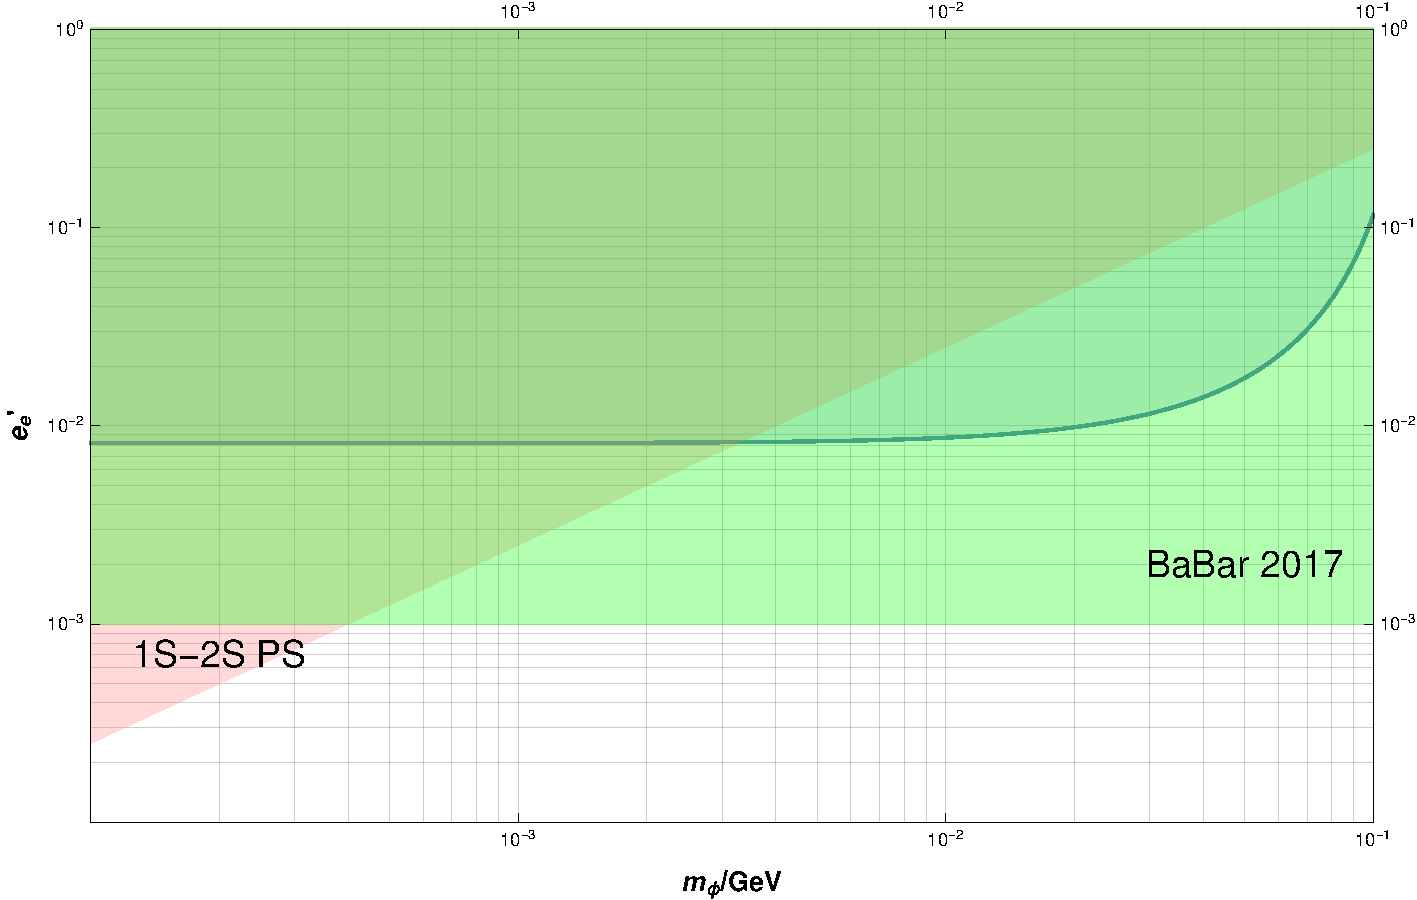
\includegraphics[width=0.8\textwidth]{imgs/LeptonUniversality}
    \caption{95\% C.L. bounds on the scalar coupling to the electron based on $R^\pi_{e/\mu}$(blue shaded) with BABAR bounds (green) and 1S-2S transitions in positronium (red)}
    \label{fg:PiSpectrumScalarUniversalityBounds}
\end{figure}
\section{Discussion}
The constraints from the removal of the chiral suppression are shown in figure \ref{fg:PiSpectrumScalarUniversalityBounds} and are again weaker than the existing bounds form BABAR. The result presented here can be generalised to $e_e'<0.008$ for $m_\phi < \SI{14}{\mega\eV}$ so even for smaller masses than shown here this bound applies. Even if the experimental precision matches the precision of the theoretical prediction, this would still not be competitive with the BABAR results.
\section{Combined Results}
\begin{figure}[ht]
  \centering
    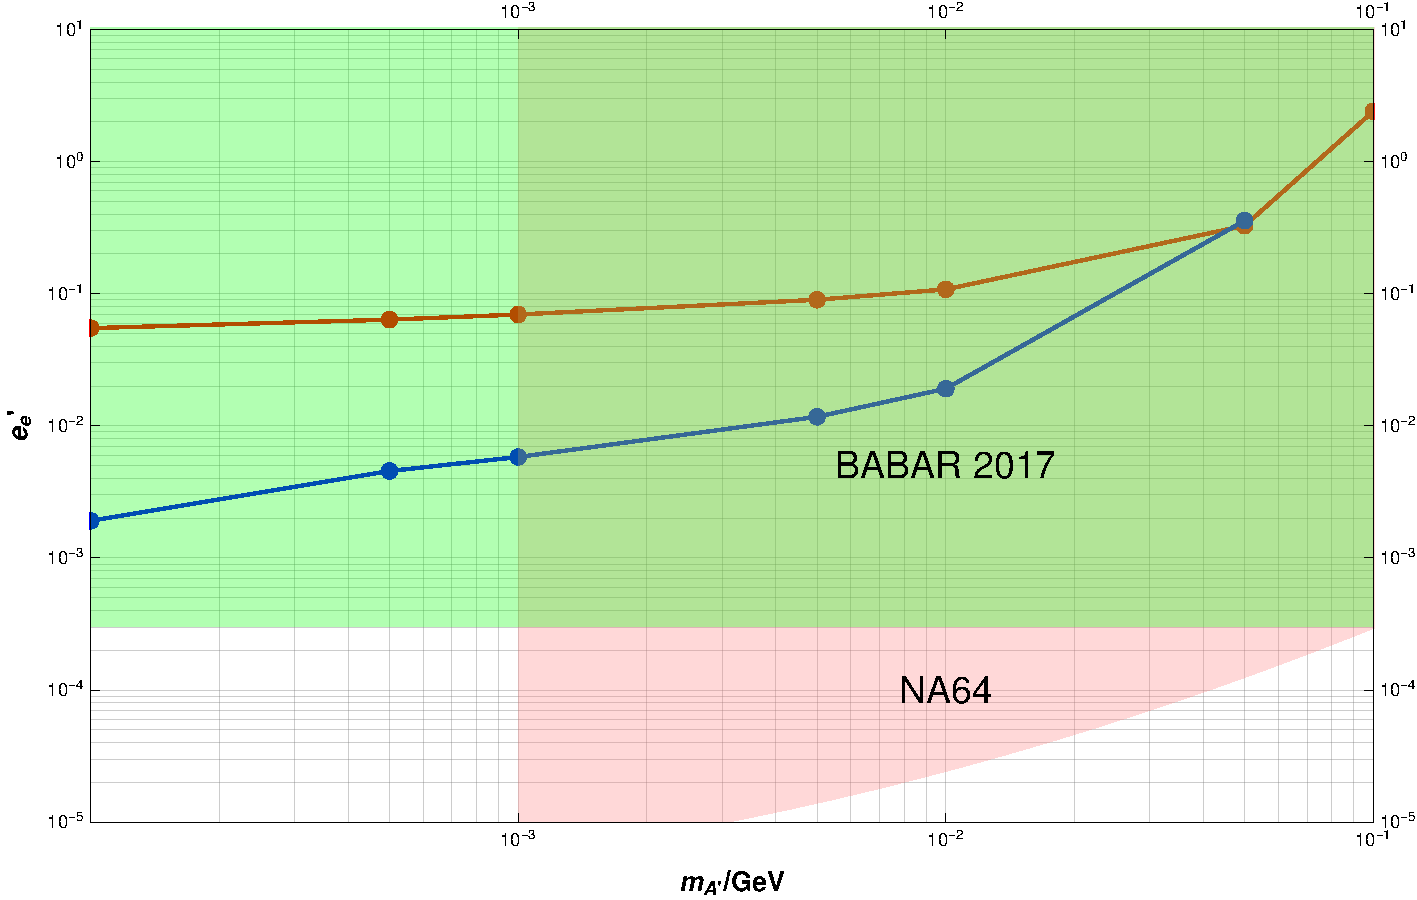
\includegraphics[width=0.8\textwidth]{imgs/combinedVector.pdf}
    \caption{95\% C.L. bounds on the vector mediator- electron coupling from the pion decay spectrum (red), the muon decay spectrum (blue), BABAR (green) and NA64 (pink)}
    \label{fg:PiMuCombinedVector}
\end{figure}

\begin{figure}[ht]
  \centering
    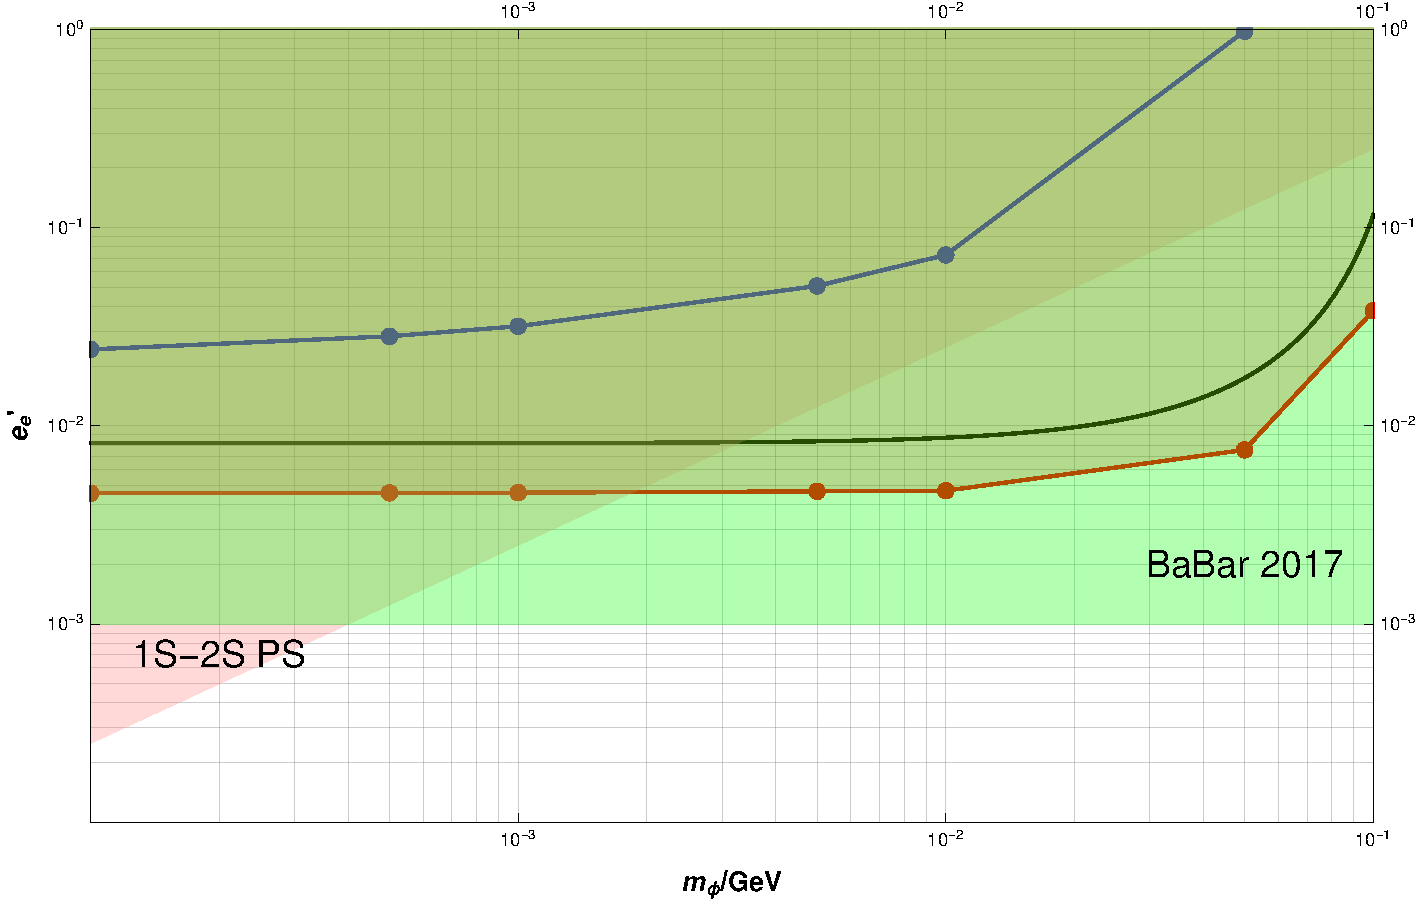
\includegraphics[width=0.8\textwidth]{imgs/combinedScalar.pdf}
    \caption{95\% C.L. bounds on the scalar mediator- electron coupling from pion decay spectrum (red), lepton universality in pion decays (smooth black line), the muon decay spectrum (blue), BABAR (green) and 1S-2S transition in positronium (pink)}
    \label{fg:PiMuCombinedScalar}
\end{figure}

Figure \ref{fg:PiMuCombinedVector} shows the combined results of both methods of constraining the parameter space of the vector mediator. In this case the analysis of the muon decay spectrum produces the stronger bounds. Despite not producing new bounds, future experimental results might produce competitive results using this method at least for light mediators.
Figure \ref{fg:PiMuCombinedScalar} shows the combined result for the scalar coupling to the electron. This time the muon results are considerably weaker than for the pion. 